\documentclass[a0paper,portrait]{baposter}


\usepackage{wrapfig}
\usepackage{lmodern}
\usepackage{xcolor}

\usepackage[utf8]{inputenc} %unicode support
\usepackage[T1]{fontenc}


\selectcolormodel{cmyk}

\graphicspath{{figures/}} % Directory in which figures are stored


\newcommand{\compresslist}{%
\setlength{\itemsep}{0pt}%
\setlength{\parskip}{1pt}%
\setlength{\parsep}{0pt}%
}

\newenvironment{boenumerate}
  {\begin{enumerate}\renewcommand\labelenumi{\textbf\theenumi.}}
  {\end{enumerate}}

\usepackage{amsmath}
\usepackage{palatino}
\usepackage{mathpazo}
\usepackage{fontawesome}
\usepackage{hyperref}

\newcommand{\mail}		[1]{\faEnvelope \quad {#1}}
\newcommand{\github}	[1]{\faGithub \quad {#1}}


\begin{document}


\definecolor{Black}{RGB}{0,0,0}
\definecolor{White}{RGB}{255,255,255}

% Basic colors
\definecolor{SeaGreen}{RGB}{111,189,165}
\definecolor{Cyan}{RGB}{0,166,214}
\definecolor{DarkBlue}{RGB}{34,70,122}
\definecolor{Purple}{RGB}{36,46,131}
\definecolor{Turquoise}{RGB}{50,154,179}
\definecolor{SkyBlue}{RGB}{130,187,206}

% Accent colors
\definecolor{Lavender}{RGB}{121,150,180}
\definecolor{Orange}{RGB}{216,130,62}
\definecolor{WarmPurple}{RGB}{110,50,122}
\definecolor{Fuchsia}{RGB}{178,72,146}
\definecolor{BrightGreen}{RGB}{183,200,34}
\definecolor{Yellow}{RGB}{247,234,151}
\definecolor{Pink}{RGB}{138,75,129}
\definecolor{Purple}{RGB}{69,48,117}

\definecolor{customBlockColor}{RGB}{111,189,165}
\definecolor{customAlertColor}{RGB}{31,112,173}
\newcommand{\mR}{\mathbb{R}}
\begin{poster}
{
grid=false,
headerborder=open, % Adds a border around the header of content boxes
colspacing=1em, % Column spacing
bgColorOne=white, % Background color for the gradient on the left side of the poster
bgColorTwo=white, % Background color for the gradient on the right side of the poster
borderColor=WarmPurple, % Border color
headerColorOne=Pink, % Background color for the header in the content boxes (left side)
headerColorTwo=Pink, % Background color for the header in the content boxes (right side)
headerFontColor=white, % Text color for the header text in the content boxes
boxColorOne=white, % Background color of the content boxes
textborder=rounded, %rectangle, % Format of the border around content boxes, can be: none, bars, coils, triangles, rectangle, rounded, roundedsmall, roundedright or faded
eyecatcher=false, % Set to false for ignoring the left logo in the title and move the title left
headerheight=0.11\textheight, % Height of the header
headershape=rounded, % Specify the rounded corner in the content box headers, can be: rectangle, small-rounded, roundedright, roundedleft or rounded
headershade=plain,
headerfont=\Large\textsf, % Large, bold and sans serif font in the headers of content boxes
textfont=\textsf, % Uncomment for paragraph indentation
linewidth=2pt % Width of the border lines around content boxes
}
{}
%
%---------------------------------------------------------------------------
%	TITLE AND AUTHOR NAME
%---------------------------------------------------------------------------
%
{
\color{WarmPurple}\textsf %Sans Serif
{Cooperative Data-Driven Modeling}
} 
%
{\sf\vspace{0.5em}\\
Aleksandr Dekhovich**, O. Taylan Turan*, Jiaxiang Yia** and Miguel A. Bessa*** 
\vspace{0.1em}\\
\small{*Pattern Recognition Laboratory, Delft University of Technology, Van Mourik Broekmanweg 6, Delft 2628 XE, The Netherlands \\
**Department of Material Science and Engineering, Delft University of Technology, Mekelweg 2, Delft, 2628 CD, The Netherlands \\
***School of Engineering, Brown University, 184 Hope St., Providence, RI 02912, US
}
\large{
\vspace{0.2em}\\
 \color{WarmPurple}\mail{o.t.turan@tudelft.nl} 
\hspace{0.2em}
  \github{github.com/taylanot}}
}
%
{}

\headerbox{1. Introduction}{name=intro,column=0,row=0, span=2}
{
  \begin{itemize}
    \color{Pink} \item \color{Black} Continual-Learning: leverages similar learning problems (tasks) for a specific similar data-scarce target learning problem (task) in a setting where the tasks are observed consequently.
  \color{Pink} \item AIM: Learning Constitutive Laws sequentially without catastrophic forgetting with Artificial Neural Networks.
  \end{itemize}
  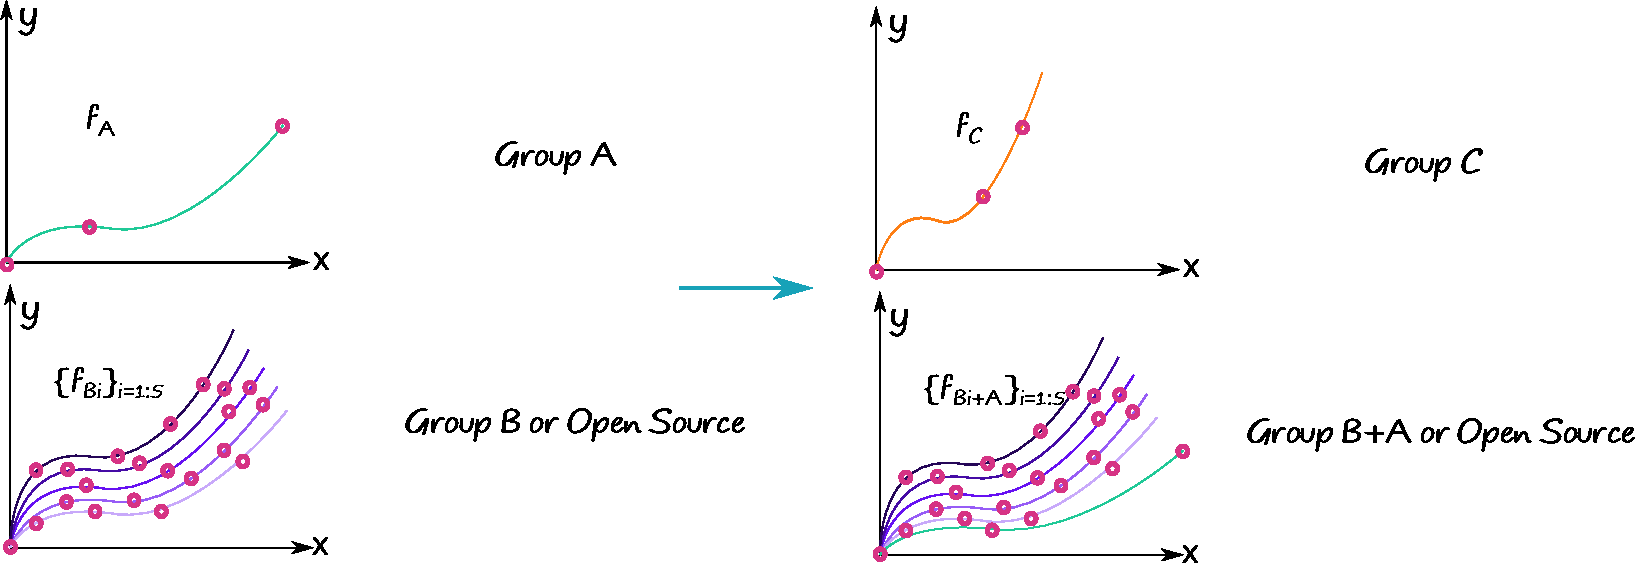
\includegraphics[width=\textwidth]{figures/aim.pdf}
}

\headerbox{3. NNRelief\cite{dekhovich2022d}}{name=prune,column=2, span=1}
{
  \begin{itemize}
    \item Train your NN for a task of $f:\mathcal{X}\to\mathcal{Y}$
    \item Compute the importance scores of the activations
    \item Prune them with a pre-defined tolerance
  \end{itemize}
  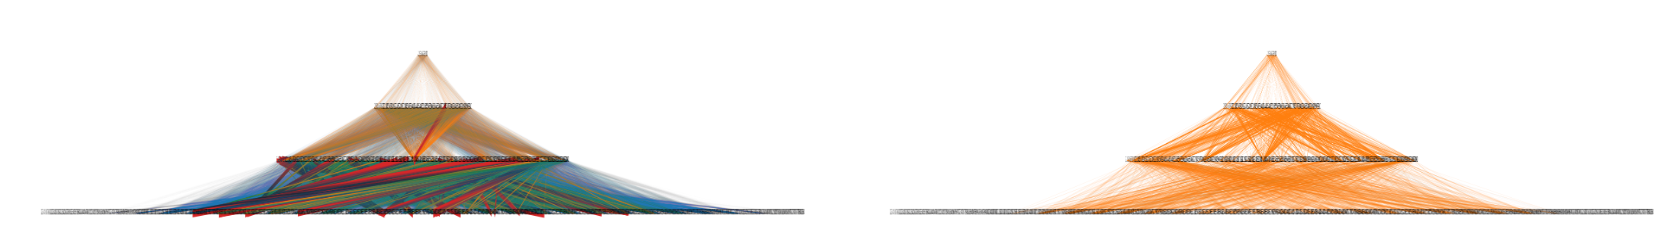
\includegraphics[width=\textwidth]{figures/nnrelief.png}
  \color{Pink} Get-rid off redundant connections $\to$ decrease parameter overload. 
}

\headerbox{2. Continual Prune \& Select\cite{dekhovich2023}}{name=cont,column=0, below=intro, span=2}
{
  \begin{minipage}{0.5\textwidth}
  \begin{itemize}
    \item Given a task $f_i:|\mathcal{X}\to\mathcal{Y}$ find sub-network $\mathcal{N}_i$ inside a given NN $\bigcup_{i=1}^M \mathcal{N}_i $
    \item Prune with NNRelief Method
    \item Fix the sub-network parameters and repeat the same procedure for $f_{i+1}$
    \item In the end you end up with task specific networks 
  \end{itemize}
  \end{minipage}%
  \begin{minipage}{0.5\textwidth}
    \centering
    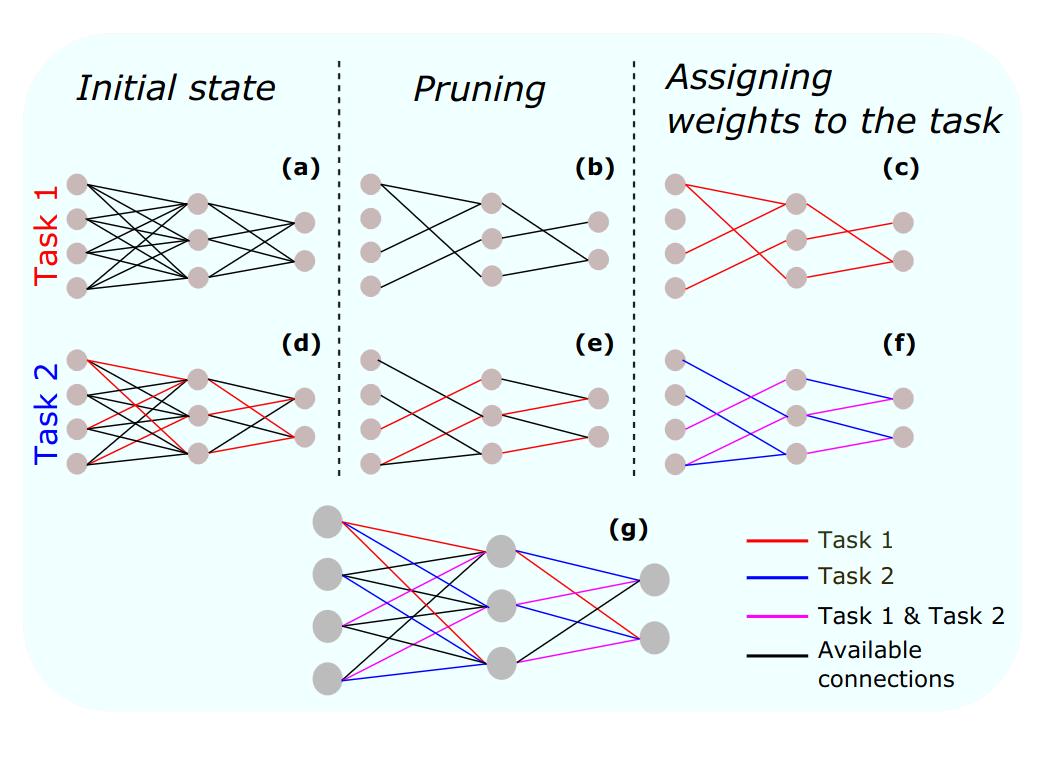
\includegraphics[width=\textwidth]{figures/pands.png}
  \end{minipage}
}


\headerbox{4. Learning Plastic Constitutive Models}{name=plastic,column=0, below=cont, span=3}
{
  \begin{minipage}{0.5\textwidth}
    \begin{itemize}
      \item Von Misses Plasticity with changing geometries 
      \item Continual Prune \& Select with GRU's
    \end{itemize}
    \centering
    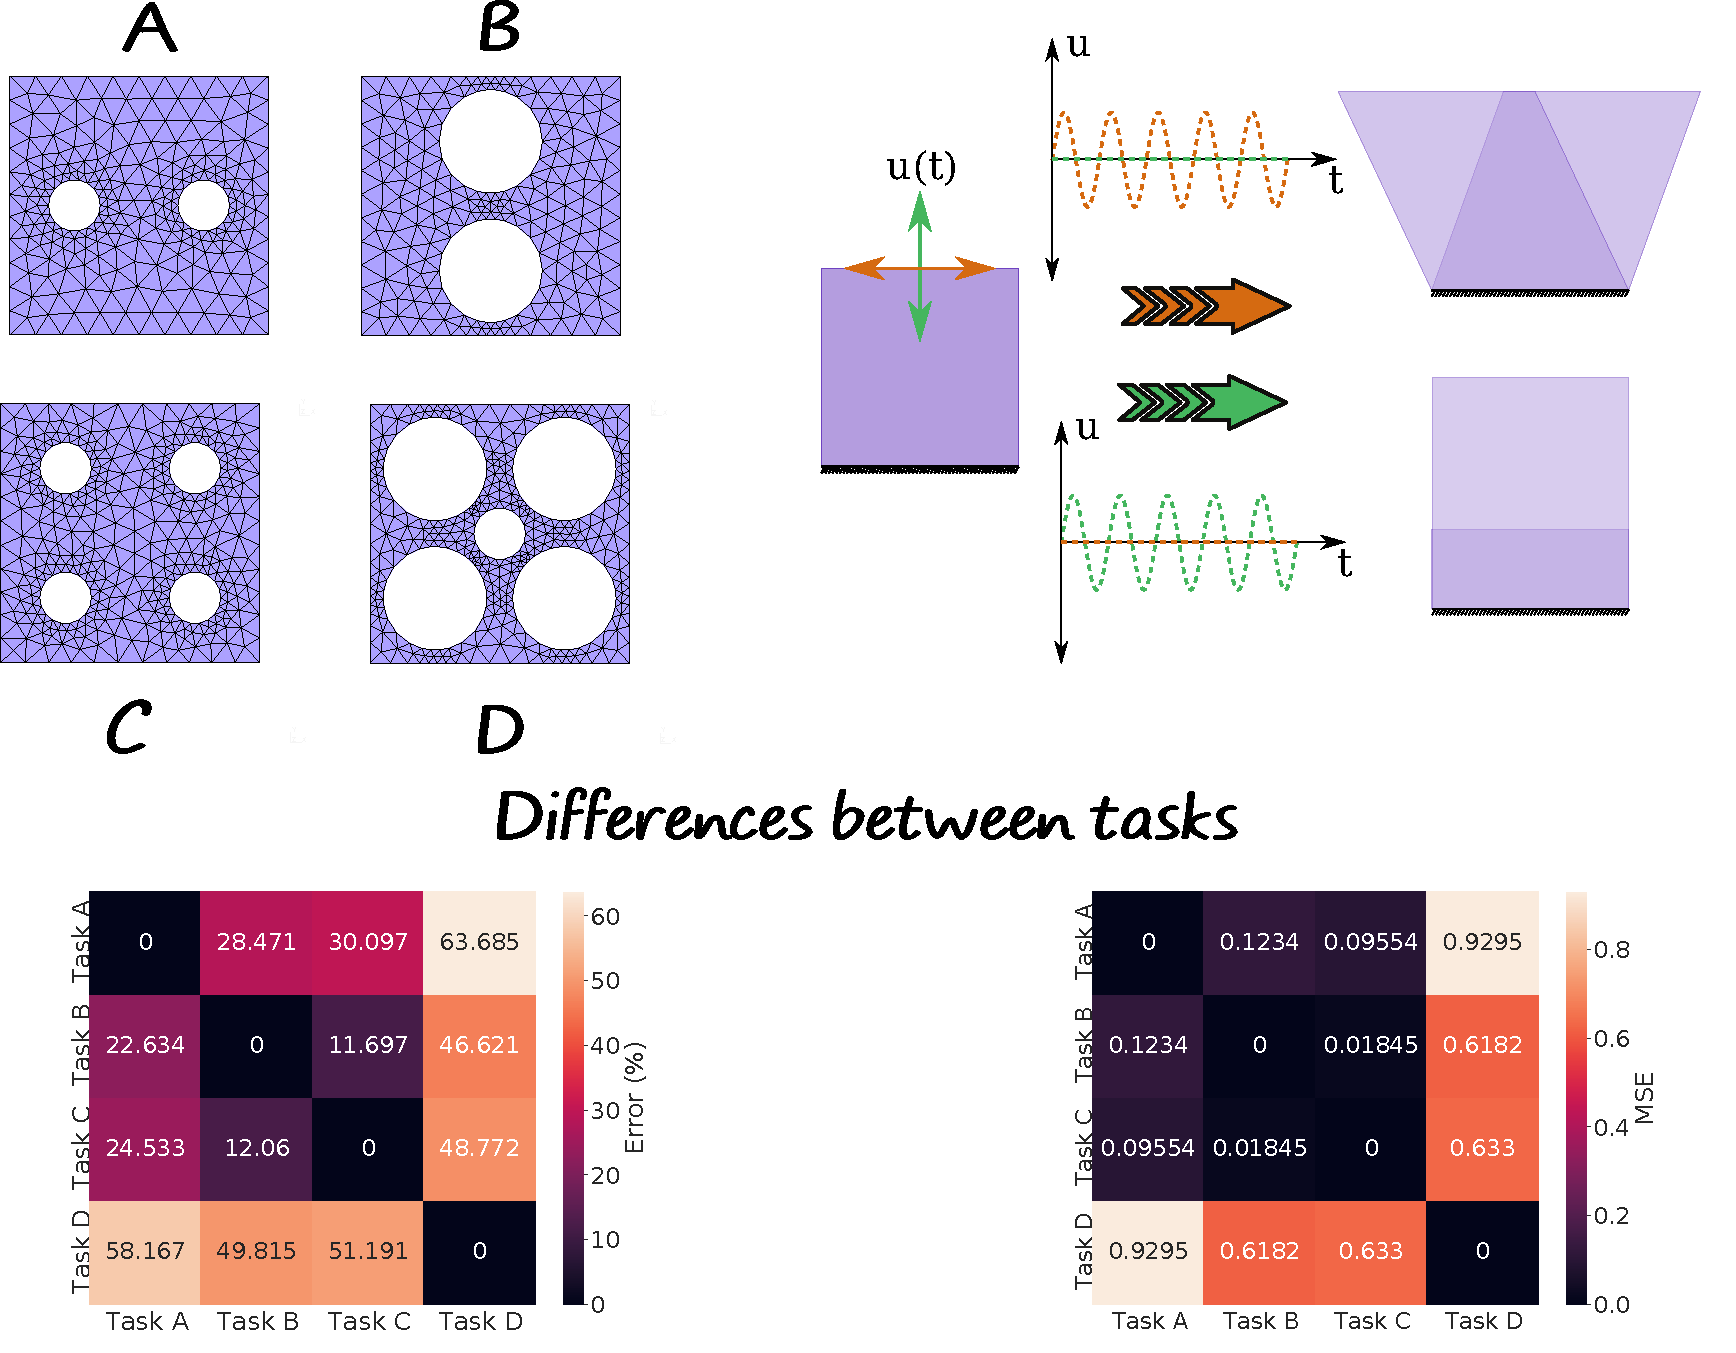
\includegraphics[width=0.8\textwidth]{figures/problem.pdf}
  \end{minipage}%
  \begin{minipage}{0.5\textwidth}
    \centering
    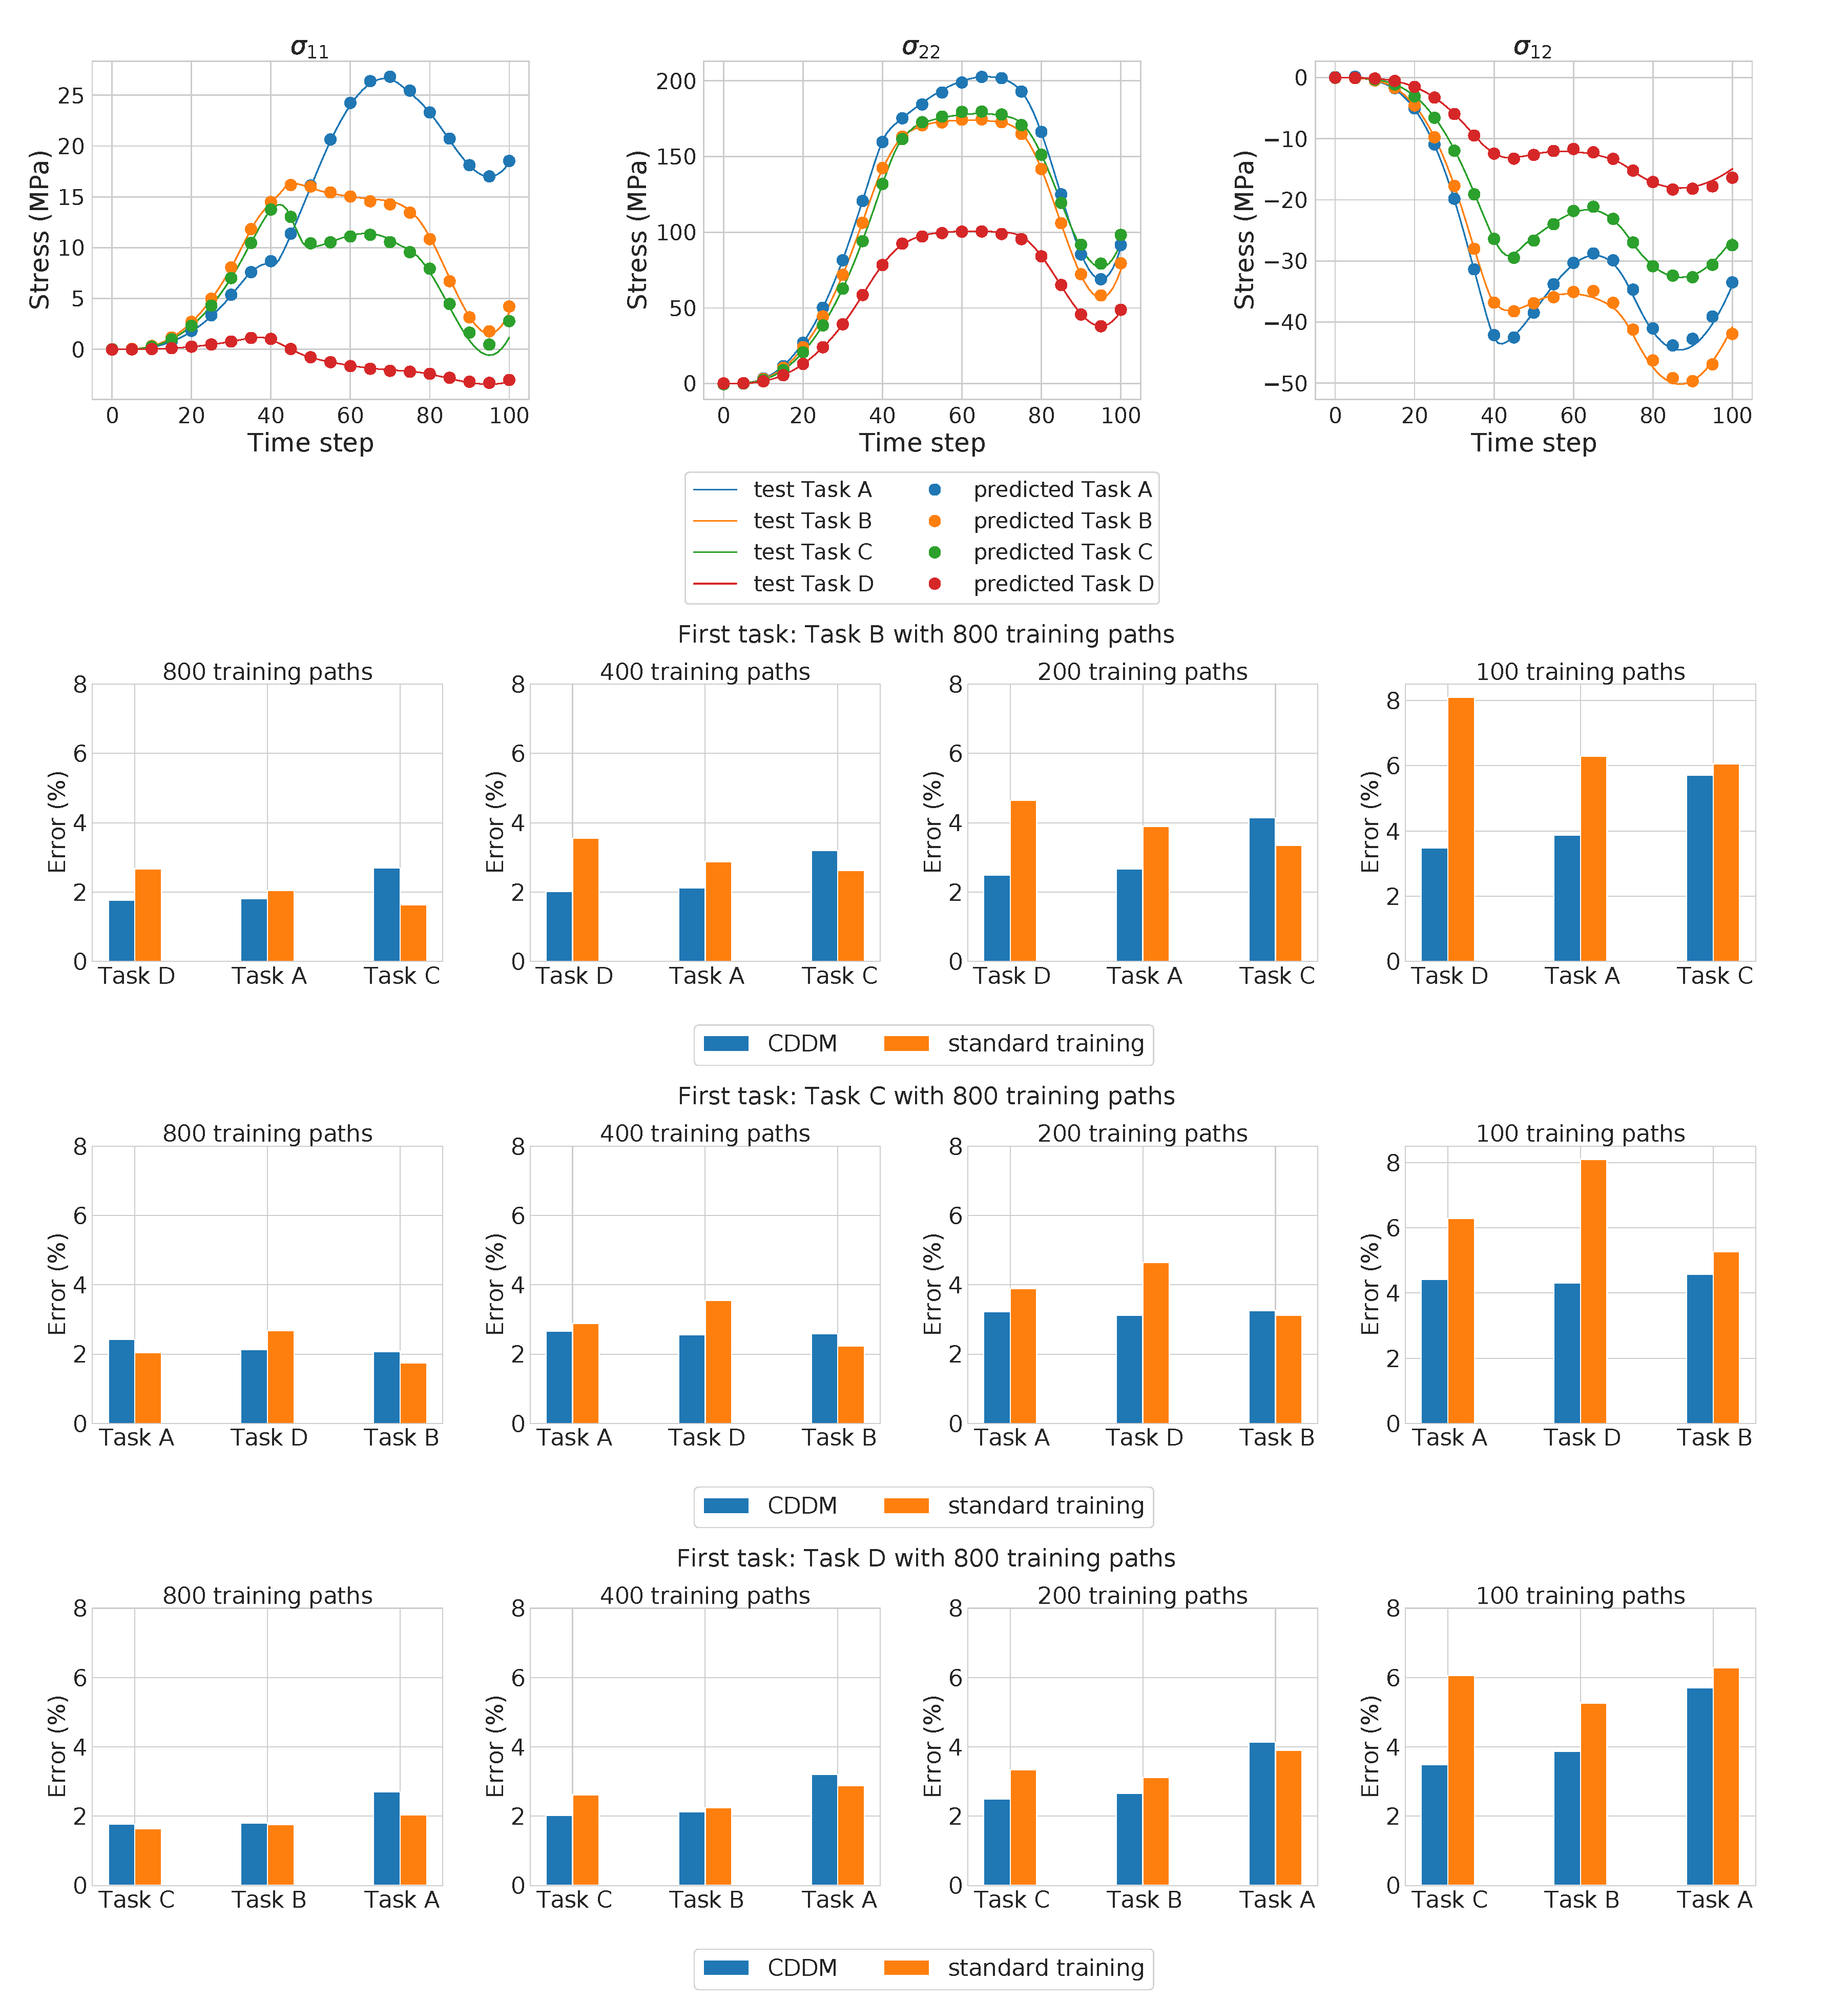
\includegraphics[width=0.7\textwidth]{figures/results.pdf}
  \end{minipage}
}

\headerbox{5. Plasticity}{name=plast,column=2, below=prune, span=1}
{
  Plastic Constitutive Law:
  \begin{itemize}
    \item Path dependent problem
    \item $\boldsymbol{\sigma}=\mathcal{C}(\epsilon, t, \boldsymbol{\theta})$ with $\sigma\in\mathbb{R}^3$ and $\epsilon\in\mathbb{R}^3$
  \end{itemize}
  As a continual learning problem:
  \begin{itemize}
    \item $\boldsymbol{\theta}$ Determines the different tasks
    \item Try to learn $\mathcal{C}$
    \item Given $\{\boldsymbol{\sigma}^{\boldsymbol{\theta_i}}_{t=1:T},\boldsymbol{\epsilon}^{\boldsymbol{\theta_i}}_{t=1:T}\}_i=1,M$
  \end{itemize}
}
\headerbox{6. Conclusions}{name=conc,column=2, below=plast, span=1}
{
  \centering
  \begin{itemize}
    \item Less number of parameters compared to standard learning.
    \item Better performance with less data.
    \item Sequential learning problem with transfer learning can enable cooperative data-driven modeling.
  \end{itemize}
}
\headerbox{7. References}{name=ref,column=0, below=plastic, span=3}
{
\renewcommand{\section}[2]{\vskip 0.05em} % Get rid of the default "References" section title
%%\nocite{*} % Insert publications even if they are not cited in the poster
\bibliographystyle{unsrt}  
\small\bibliography{/home/taylanot/Dropbox/archive_bib/aleksandr_colab.bib}   

}
%\headerbox{5.Learning Curve Application
%}{name=lc,column=0, below=res, span=2}
%{
%  \begin{minipage}{0.5\textwidth}
%    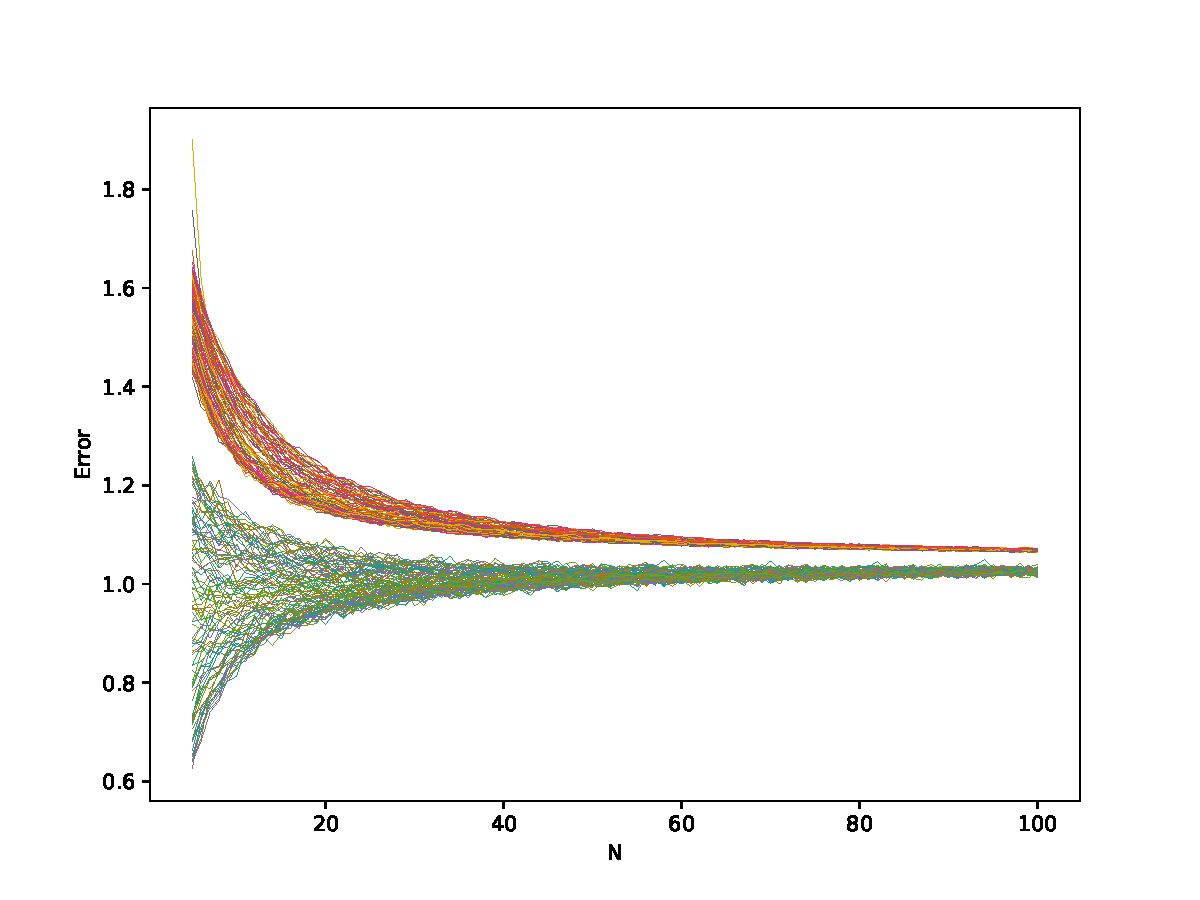
\includegraphics[width=\textwidth]{figures/lr_learning_curves.pdf}
%  \end{minipage}%
%  \begin{minipage}{0.5\textwidth}
%    \begin{itemize}
%      \item Bunch of learning curves for varying regularization $\lambda$
%      \item Work in progress!!!
%    \end{itemize}
%  \end{minipage}
%}
%\headerbox{5. Ridge Regression Learning Curve Application  
%}{name=lc,column=0, below=res, span=1}
%{
%
%  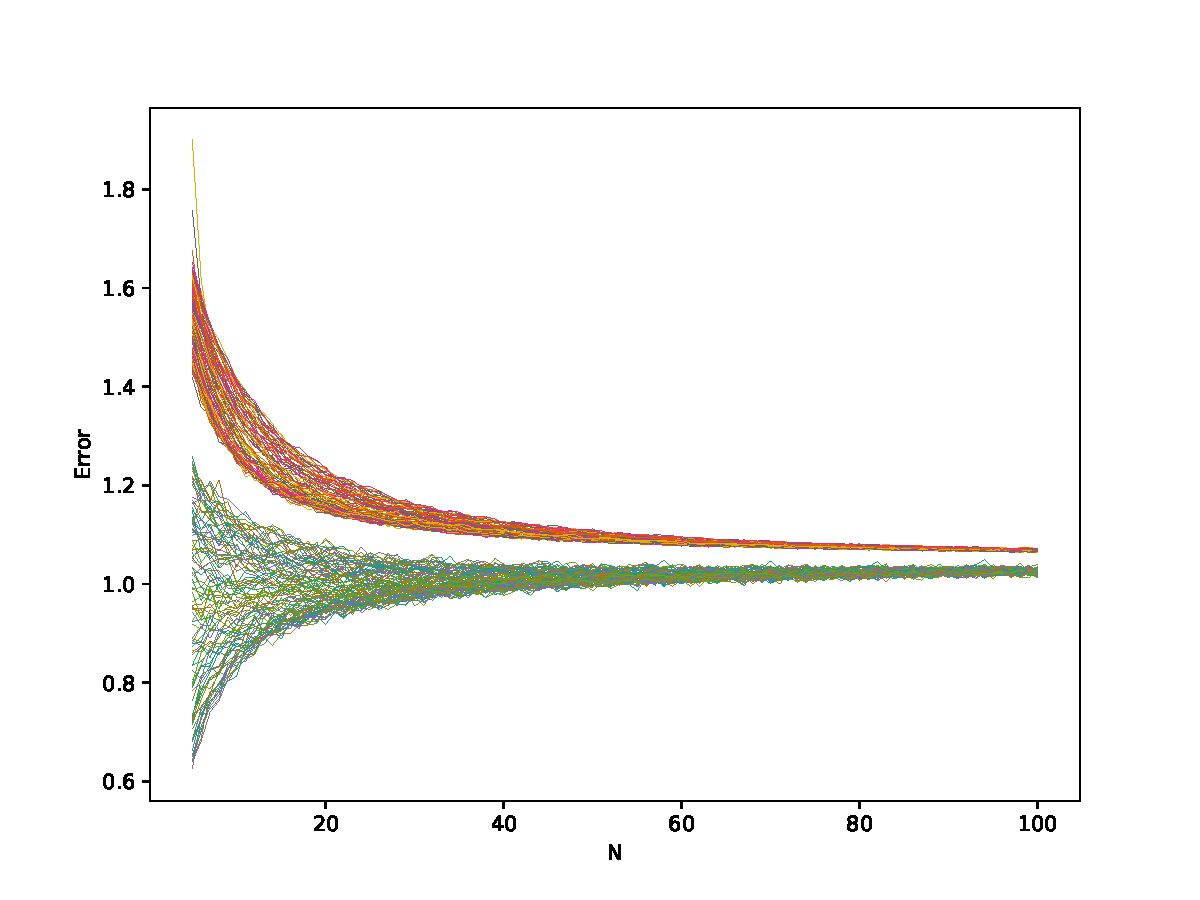
\includegraphics[width=\textwidth]{figures/lr_learning_curves.pdf}
%}
\end{poster}

\end{document}
